As discussed in Section~\ref{sec:related_works}, MTLNet \cite{silva2025mtlnet} uses a single vector $\mathbf{E}_{DGI} \in \mathbb{R}^{64}$ as input for both tasks, jointly encoding spatial and categorical information through the graph topology. One limitation of this monolithic approach is that it does not incorporate continuous geographic coordinates or temporal visitation patterns, factors that, as shown by works on spatial \cite{wu2024torchspatial} and temporal \cite{kazemi2019time2vec} encoding, carry information complementary to the topological relationships of the graph.

The central design decision of this work is to decompose the unimodal DGI representation into three independent 64-dimensional components, trained separately and integrated by concatenation: a continuous spatial \textit{encoder}, a temporal \textit{encoder} (Time2Vec), and a hierarchical categorical \textit{encoder} (HGI). The underlying hypothesis is that a decoupled representation, with specialized \textit{encoders} trained with loss functions suited to each dimension of the information, produces more expressive representations than a unimodal representation that encodes all dimensions jointly. To evaluate this hypothesis and investigate the impact of the spatial encoding strategy, two \textit{encoders} with distinct architectural assumptions are compared: SIREN and Sphere2Vec-M.

The proposed methodology is illustrated in Figure~\ref{fig:arquitetura_arch}. The following describes the MTLNet model, the \textit{baseline} with DGI, the rationale and operation of each proposed \textit{encoder}, and the strategy for integrating the \textit{embeddings}.


\begin{figure*}[htbp]
    \centering
    \makebox[\textwidth][c]{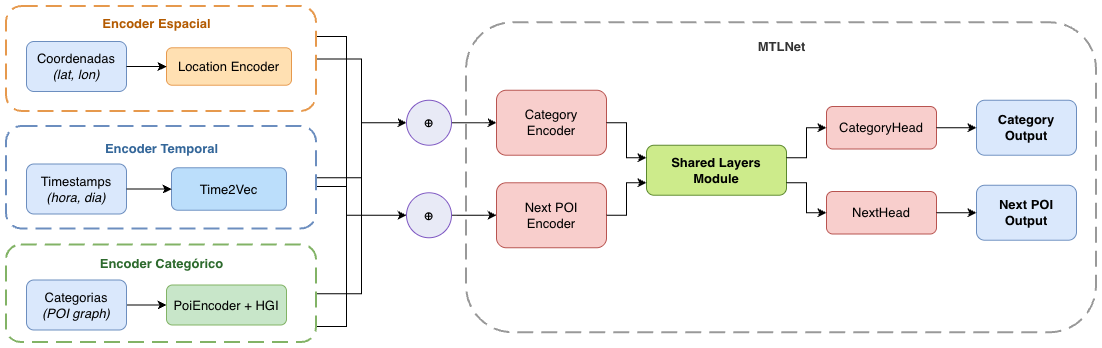
\includegraphics[width=1\textwidth]{imagens/arquitetura_modelo.png}}
    \caption{Architecture based on MTLNet \cite{silva2025mtlnet}. The spatial, temporal, and categorical \textit{encoders} are trained in a decoupled manner and generate their respective \textit{embeddings}, which are integrated as input to the model and processed by the model's shared layers (\textit{Shared Layers Module}) and by the task-specific layers, producing the \textit{Category Output} and \textit{Next POI Output}.}
    \label{fig:arquitetura_arch}
\end{figure*}

MTLNet \cite{silva2025mtlnet} is a multi-task network built on hard parameter sharing \cite{caruana1997multitask}, which simultaneously processes the POI Category Classification and Next-POI Prediction tasks. The architecture uses task-specific \textit{encoders} implemented as MLPs with LayerNorm and Dropout, which project the input \textit{embeddings} into a shared latent space of dimension $d_{\mathrm{shared}} = 256$. Next, FiLM modulation (\textit{Feature-wise Linear Modulation}) \cite{perez2018film} is applied, conditioned by a task-identifier \textit{embedding} $\mathbf{e}_{t}$, which generates scale $\gamma_{t}$ and shift $\beta_{t}$ parameters to modulate the encoded representations:

\begin{equation}
\mathrm{FiLM}(\mathbf{h}_{\mathrm{enc}}^{(t)} \,|\, \mathbf{e}_{t}) = \gamma_{t} \odot \mathbf{h}_{\mathrm{enc}}^{(t)} + \beta_{t}
\label{eq:film}
\end{equation}

The modulated representations are processed by four shared residual blocks with LayerNorm, LeakyReLU, and Dropout, allowing the model to learn a common representation for both tasks \cite{baxter2000model}.

At the output, each task has a specialized \textit{head}. The category classification module uses a set of three parallel MLPs with varying depths (2, 3, and 4 layers), whose outputs are concatenated and projected to the 7 POI classes. The next-POI \textit{head} employs a \textit{Transformer encoder} with 8 attention \textit{heads} and 4 layers, a causal mask for autoregressive processing, and attention-weighted pooling using attention weights learned over the \textit{timesteps} of the input sequence. %(janela de tamanho $L_h = 9$).

Multi-task training uses the Nash-MTL regularizer \cite{nash}, which formulates gradient balancing as a cooperative Nash bargaining game among $K$ tasks. Given the gradients of each task, Nash-MTL seeks the update direction that maximizes the product of the utilities of all tasks, which ensures that the update is beneficial for all tasks simultaneously, avoiding the dominance of one task over the other.


% \begin{equation}
% \Delta\boldsymbol{\theta}^{*} = \arg\max_{\Delta\boldsymbol{\theta} \in \mathcal{B}_\varepsilon}
% \sum_{k=1}^{K} \log\!\left(\mathbf{g}_k^{\top} \Delta\boldsymbol{\theta}\right)
% \quad\text{s.t. } \mathbf{g}_k^{\top} \Delta\boldsymbol{\theta} > 0,\;\forall k
% \label{eq:nash}
% \end{equation}

\subsection{Baseline: MTLNet with DGI}

The \textit{baseline} model corresponds to the original MTLNet proposed in \cite{silva2025mtlnet}, whose internal architecture is kept unchanged in this work. In this model, each POI is represented by a single monolithic \textit{embedding} $\mathbf{E}_{DGI} \in \mathbb{R}^{64}$, obtained via \textit{Deep Graph Infomax} (DGI) \cite{velickovic2019deep} over a spatial graph built by Delaunay triangulation and categorical node attributes, as described in detail in \cite{silva2025mtlnet}. Thus, DGI jointly encodes spatial and categorical relationships in a single vector, without incorporating explicit temporal components. In contrast, the proposed approach replaces this monolithic representation with the concatenation of three specialized \textit{encoders}, totaling 192 input dimensions.


\subsection{Data Preparation}

For the \textit{POI Category Classification} task, each POI is represented by the \textit{embedding} resulting from the concatenation of the three components, $\mathbf{E}_{cat} = [\mathbf{E}_{HGI} \| \mathbf{E}_{loc} \| \mathbf{E}_{time}] \in \mathbb{R}^{192}$, forming pairs $(\mathbf{E}_{cat}, c)$ where $c$ is the real category of the POI. In the case of the \textit{baseline}, $\mathbf{E}_{DGI} \in \mathbb{R}^{64}$ is used directly.

For the \textit{Next-POI Prediction} task, the \textit{check-ins} are ordered chronologically per user, and users with fewer than five visits are discarded. Non-overlapping windows of size $L_h = 9$ are extracted: the \textit{check-ins} $(p_1, \dots, p_9)$ form the context, and $p_{\text{target}}$ is the next POI whose category must be predicted. Each \textit{check-in} in the window is represented by the corresponding \textit{embedding}, resulting in an input of $9 \times 192 = 1728$ dimensions for ST-MTLNet and $9 \times 64 = 576$ dimensions for the \textit{baseline}. Shorter sequences are filled with padding of zero vectors.

\subsection{Spatial Encoder}

The original MTLNet model encodes spatial information implicitly through the topology of the Delaunay graph, without directly using geographic coordinates as an input signal. However, as discussed in Section~\ref{sec:related_works}, continuous spatial encoders have shown effectiveness in various geospatial tasks \cite{wu2024torchspatial}, although their application in multi-task POI models remains little explored. This work selects two \textit{encoders} that represent distinct spatial encoding paradigms: SIREN \cite{rußwurm2024geographiclocationencodingspherical}, which models continuous functions through sinusoidal activations with controllable frequencies, and Sphere2Vec-M \cite{mai2023sphere2vecgeneralpurposelocationrepresentation}, which operates directly on spherical coordinates preserving geodesic distance properties. This diversity allows evaluating how different geometric and architectural assumptions impact performance on POI tasks.

All \textit{encoders} produce $\mathbf{E}_{loc} \in \mathbb{R}^{64}$ and are
trained with the same binary contrastive loss based on the geographic distance between pairs of coordinates:
\begin{equation}
\mathcal{L}_{\text{loc}}(i,j)
=
- \left[
y_{ij}\,\log \sigma\!\left(\frac{\text{sim}(z_i,z_j)}{\tau}\right)
+
(1-y_{ij})
\log \left(1 - \sigma\!\left(\frac{\text{sim}(z_i,z_j)}{\tau}\right)\right)
\right]
\end{equation}

in which $\sigma$ denotes the sigmoid function, $\text{sim}(\cdot,\cdot)$ is the cosine similarity, and $y_{ij} \in \{0,1\}$ indicates whether the pair is positive ($\Delta d_{ij} \leq 10$ km) or negative ($\Delta d_{ij} \geq 70$ km), with temperature $\tau = 0.15$. Using the same loss function for the two spatial \textit{encoders} allows a controlled comparison, isolating the effect of the encoding architecture.

% \subsubsection{Space2Vec-grid}

% O Space2Vec-grid proposto por Mai et al. \cite{mai2020multiscalerepresentationlearningspatial} realiza a modelagem espacial a partir das coordenadas contínuas de latitude e longitude dos \textit{check-ins} e pode ser definido em duas camadas principais:

% \begin{description}
%     \item[\textbf{Codificador Posicional Senoidal (\textit{Position Encoder}):}]
%     As coordenadas ($\lambda, \phi$) dos \textit{check-ins} são transformadas em um vetor de alta dimensão por meio de funções senoidais e cossenos com frequências logaritmicamente espaçadas.

%     \item[\textbf{Rede Neural \textit{Feed-Forward} (FFN):}]
%     O vetor de codificação posicional é processado por uma FFN de múltiplas camadas com \textit{skip connection} e LayerNorm, que projeta a representação no \textit{embedding} final $\mathbf{E}_{loc} \in \mathbb{R}^{64}$.
% \end{description}

\subsubsection{SIREN}

The SIREN model (\textit{Sinusoidal Representation Networks}) \cite{rußwurm2024geographiclocationencodingspherical} models a continuous function $f_\theta : \mathbb{R}^2 \rightarrow \mathbb{R}^{64}$ that directly maps normalized geographic coordinates into a vector \textit{embedding}. Each layer of the network uses sinusoidal activations with controllable frequencies, allowing high-frequency signals in spatial data to be represented. The output is the \textit{embedding} $\mathbf{E}_{loc} \in \mathbb{R}^{64}$.

\subsubsection{Sphere2Vec-M}

Sphere2Vec-M \cite{mai2023sphere2vecgeneralpurposelocationrepresentation} is a multi-scale encoder formulated to operate directly on spherical coordinates ($\lambda$, $\phi$), generating representations that preserve distance properties on the surface of the sphere. The \textit{sphereM} variant is used, in which $S=16$ multi-resolution scales are employed with geometrically spaced factors between 10 km and 10,000 km. Interaction terms between $\lambda$ and $\phi$ are constructed by keeping one of the components at the highest scale level, allowing the angular resolution of latitude and longitude to be controlled independently. The resulting vector is projected by an MLP to produce $\mathbf{E}_{loc} \in \mathbb{R}^{64}$.

\subsection{Temporal Encoder}

Human mobility patterns exhibit cyclical regularities, such as meal times and weekly movements, which carry discriminative information about the functional nature of the visited POIs \cite{sun2020go}. However, the original MTLNet model does not incorporate explicit temporal representations to capture this information.

To fill this gap, Time2Vec \cite{kazemi2019time2vec} is used, a generic and decoupled temporal representation capable of capturing periodic and non-periodic patterns without the need for manual feature engineering. The architecture combines linear and periodic terms to map the temporal values of each \textit{check-in} (hour of day and day of week, in a coupled manner) into an \textit{embedding} vector. For an \textit{embedding} of dimension $D$, the function is defined as:

\begin{equation}
\mathbf{f}(\tau)[i] = \begin{cases} \omega_0 \tau + \phi_0 & \text{if } i=0 \\ \sin(\omega_i \tau + \phi_i) & \text{if } 1 \leq i \leq D-1 \end{cases}
\label{eq:time2vec}
\end{equation}

in which $\omega_i$ and $\phi_i$ are trainable parameters (weights and \textit{bias}) that capture the periodicity of the temporal visitation patterns. The linear term ($i=0$) captures global temporal trends, while the sinusoidal terms model cyclical patterns at different frequencies.

The model is trained using the discrete temporal values (hour of day and day of week) in a coupled manner for each \textit{check-in}, with the same binary contrastive formulation employed in the spatial encoder, denoted $\mathcal{L}_{tempo}$. The final output is the \textit{embedding} $\mathbf{E}_{time} \in \mathbb{R}^{64}$, which represents the \textit{timestamp} of each \textit{check-in}.

\subsection{Categorical Encoder}

The DGI used in the original model encodes categorical information through a \textit{one-hot} matrix of 7 classes processed by the graph structure, without explicitly capturing hierarchical or regional relationships among POI categories. To enrich this dimension, the generation of categorical \textit{embeddings} is carried out in two complementary phases. The POI Encoder learns vector representations that capture co-occurrences among categories from random walks on the spatial graph, and the HGI model \cite{huang2023learning} incorporates hierarchical information at multiple levels (POI, region, and city), producing representations that reflect both the local and the regional context.

\subsubsection{POI Encoder}

The POI Encoder is trained independently to generate the category \textit{embedding} $\mathbf{E}_{\text{POI\_category}} \in \mathbb{R}^{64}$. The POIs are organized into a spatial graph built by Delaunay triangulation over the geographic coordinates, with edges weighted by logarithmic decay of the Haversine distance and penalization for connections between distinct counties (GEOIDs).

Over this graph, random walks (\textit{random walks}) are executed following the Node2Vec methodology \cite{grover2016node2vec}. Each walk is converted into a sequence of secondary categories (\textit{fclass}), resulting in local and global co-occurrences among categories. The model learns the \textit{embeddings} using the \textit{skip-gram} strategy with \textit{negative sampling} \cite{church2017word2vec}:

\[
\mathcal{L}_{\text{SGNS}}(i,j)
=
-\log \sigma\!\left(\mathbf{e}_j^\top \mathbf{e}_i\right)
-
\sum_{k=1}^{K}
\log \sigma\!\left(-\mathbf{e}_{n_k}^\top \mathbf{e}_i\right),
\]

in which $\mathbf{e}_i$ is the \textit{embedding} of the target class, $\mathbf{e}_j$ the positive context \textit{embedding}, and $\mathbf{e}_{n_k}$ represent the negative samples. The implementation incorporates a hierarchical regularization term \cite{belkin2003laplacian} between category and \textit{fclass}: $\mathcal{L}_{\text{hier}} = \sum_{(c,s) \in \mathcal{H}} \left\| \mathbf{e}_s - \mathbf{e}_c \right\|_2^2$, in which $\mathcal{H}$ contains the (category, \textit{fclass}) pairs. The total loss is $\mathcal{L} = \mathcal{L}_{\text{SGNS}} + \lambda_{\text{hier}} \, \mathcal{L}_{\text{hier}}$. In the end, the resulting \textit{embedding} is generated per category and remapped to each POI.

\subsubsection{Hierarchical Graph Infomax (HGI)}

After the generation of the \textit{embeddings} $\mathbf{E}_{\text{POI\_category}}$, they are used as input to the Hierarchical Graph Infomax (HGI) model \cite{huang2023learning}, which enriches the representation by incorporating regional geographic information. The model optimizes mutual information at two hierarchical levels (POI-region and region-city):

\[
\mathcal{L}
=
\alpha\,\mathcal{L}_{\text{POI--region}}
+
(1-\alpha)\,\mathcal{L}_{\text{region--city}},
\]

in which $\alpha = 0.5$ controls the balance between the hierarchical levels. Both losses use structural negative sampling to reinforce the separability between regions and between POIs. The output is the enriched \textit{embeddings} $\mathbf{E}_{\text{HGI}} \in \mathbb{R}^{64}$, which capture both local and regional categorical relationships.



\subsection{Embedding Integration}

The three representation components are trained independently and concatenated to form the input of both MTLNet tasks:

\begin{equation}
\mathbf{E}_{input} = [\mathbf{E}_{HGI} \| \mathbf{E}_{loc} \| \mathbf{E}_{time}] \in \mathbb{R}^{192}
\label{eq:concat}
\end{equation}

The choice of concatenation as the integration strategy preserves the individual information of each component without imposing premature interactions between the representations, delegating to MTLNet the task of learning how to combine these dimensions through its shared layers and FiLM modulation. The input dimensionality of ST-MTLNet ($\mathbb{R}^{192}$) is higher than that of the \textit{baseline} ($\mathbb{R}^{64}$), a natural consequence of the decomposition into three specialized components.

However, the MTLNet architecture projects any input to the same shared latent space of dimension $d_{\mathrm{shared}} = 256$ through the task-specific \textit{encoders}, so that the capacity of the shared layers and task heads remains unchanged across the evaluated models. Even so, the difference in input dimensionality may influence part of the observed gains. For this reason, an additional experimental control equalizing the dimensionality of the representations would allow validating more precisely whether the gains occur mainly from the semantic specialization of the \textit{encoders}, and not only from the increase in input dimensionality.

Two variants of the proposed model are evaluated, named ST-MTLNet (\textit{Spatial-Temporal MTLNet}), each using a different spatial \textit{encoder}. The \textit{baseline} MTLNet \cite{silva2025mtlnet} uses only the monolithic \textit{embedding} $\mathbf{E}_{DGI} \in \mathbb{R}^{64}$ as input for both tasks. The proposed variants replace this representation with the concatenation of the decoupled \textit{embeddings}, keeping the temporal (Time2Vec) and categorical (HGI) \textit{encoders} fixed and varying the spatial \textit{encoder} between SIREN and Sphere2Vec-M.

All models share the same hyperparameters of the MTLNet architecture, differing only in the input \textit{embeddings}. This configuration allows isolating the effect of the representation strategy on performance, evaluating both the gain of the modular approach relative to the monolithic \textit{baseline} and the impact of the choice of the spatial \textit{encoder}.